\section{A Stakeholder-First Approach to Designing Transparent ADS}
\label{sec:explain}

\subsection{Definitions}

Technologists and AI researchers have not agreed on a definition of transparency for AI systems. Instead, a number of terms have been used, including explainability, interpretability, intelligibility, understandability, and comprehensibility~\cite{DBLP:journals/corr/abs-2012-01805}. There is no consensus on the meaning of these terms and they are often defined differently by different authors or used interchangeably. Furthermore, transparency and its related terms cannot trivially be quantified or measured, and transparency for one stakeholder does not automatically imply the same for different stakeholders~\cite{lipton2018mythos, hind2019explaining}.

While having multiple definitions of transparency has been useful for distinguishing nuance in a research setting, it also poses a challenge for policy making. In contrast to technologists, policymakers favor definitions of transparency that are about human thought and behavior such as accountability or legibility~\cite{DBLP:conf/aies/KrafftYKHB20}. Table~\ref{terms} outlines terms related to transparency commonly used by policymakers versus those used by technologists.

{\bf Transparency}. For the purposes of this paper, we choose to use only the term ``transparency,'' in the broadest possible sense, so that it encompasses all the definitions above. This is most similar to the way ``explainability'' is used by technologists.  Here we use the definition adapted from work by Christoph Molnar and define transparency as ``the degree to which a human can understand an AI system~\cite{molnar2019}.'' %The nuance lost by disregarding other transparency terms will be regained through the stakeholder-first approach to transparency that constitutes the first contribution of this paper and is described next.

{\bf Explanation}. We use the term ``explanation'' to refer to an instantiation of transparency. For example, to ensure transparency for a system, a technologist may create an \emph{explanation} about the data it uses.

\begin{table}[h!]
\centering
\label{tab:data}
\small
\begin{tabular}{ cc }
\toprule
{\bf Terms used by policymakers} & {\bf Terms used by technologists} \\
\midrule
\makecell{Transparency \\ Accountability \\ Understandable \\ Legibility \\ Traceability \\ Redress} & \makecell{Explainability \\ Transparency \\ Interpretablity \\ Intellegibility \\ Understandability \\ Comprehensibility \\ Recourse} \\
\bottomrule
\end{tabular}
\caption{Discrepancies in the way policymakers and AI practitioners communicate about the transparency of AI systems.}
\end{table}\label{terms}

{\bf Automated Decision Systems.} The approach described in this paper applies to all Automated Decision Systems (ADS), which is any system that processes data to make decisions about people. This means that AI systems are a subset of ADS, but there are two key distinctions: (1) an ADS is underpinned by any algorithm and not just AI or machine learning, and (2) an ADS implies a context of use and some kind of impact. For a formal definition of ADS, see ~\cite{DBLP:journals/pvldb/StoyanovichHJ20}. Henceforth, we will use the term ADS.

Notably, while many regulations are written to specifically mention ``AI systems'', all the ideas they contain about transparency could be applied to all ADS. It is likely that future regulations will focus broadly on ADS, as seen in NYC Local Law 144 of 2021 and France's Digital Republic Act.



%broadly, of which ADS are a subset. The key difference being that while an ADS may use an ADS, it also implies a context of use and impact. Formally, ADS (1) process data about people; (2) help make decisions that are consequential to people's lives and livelihoods; (3) are designed with the stated goals of improving efficiency and promoting, or at least not hindering, equitable access to opportunity; (4) involve a combination of human and automated decision making; and (5) are subject to auditing for legal compliance and, at least potentially, to public disclosure~\cite{DBLP:journals/pvldb/StoyanovichHJ20}.

%This means that an ADS may make decisions using an AI or some simpler algorithm, but importantly, 

%AI and ADS systems may be used alone or in conjunction with humans, often referred to as having a “human-in-the-loop”.  In this case, the ADS may also be referred to as a “decision support system”, and the system will provide some information or recommendation that supports human decision making ~\cite{gillingham2019can,wagner2019liable,raso2017displacemen}.


%Central to this ADS definition is the placing of technical decision-making components---a spreadsheet formula, a matchmaking algorithm, or a predictive analytic---within the lifecycle of data collection and analysis, and within the socio-legal context of design, development, deployment, and oversight.



%Importantly, since ADS systems are prone to the same issues related to bias and fairness, discrimination, transparency, data privacy, and accountability as AI and ML systems, we make the claim that the ``right to an explanation'' should apply to all ADS.  In the rest of this paper we will take a broad interpretation of ADS, understanding  AI and ML systems as ADS components.  

\subsection{Running Example: Predicting Unemployment in Portugal}

To make the discussion concrete, we use a running example of an ADS implemented in Portugal to try and prevent long-term unemployment (being unemployed for 12 months or more). The long-term unemployed are particularly vulnerable persons, and tend to earn less once they find new jobs, have poorer health and have children with worse academic performance as compared to those who had continuous employment~\cite{nichols2013consequences}. The Portuguese national employment agency, the Institute for Employment and Vocational Training (IEFP), uses an ADS to allocate unemployment resources to at-risk unemployed persons. The system is based on demographic data about the individual, including their age, unemployment length, and profession, along with other data on macroeconomic trends in Portugal.

The ADS is used by job counselors who work at the IEFP unemployment centers spread across Portugal. This interaction model, where an ML system makes a prediction and a human ultimately makes a final determination informed by the system's predictions, is referred to as having a ``human-in-the-loop'' (HITL). Having a HITL is an increasingly common practice for implementing ADS ~\cite{gillingham2019can,wagner2019liable,raso2017displacement}. The ADS assigns unemployed persons as low, medium, or high risk for remaining unemployed, and then job counselors have the responsibility of assigning them to interventions such as re-skilling, resume building, or job search training ~\cite{zejnilovic2020algorithmic}.

%In this context, explanations were used to help job counsellors make better decisions about assigning unemployed individuals to the appropriate interventions.  Explanations were given in the following way:  counselors would see both the predicted risk category of the individual (low, medium, or high), the raw score of the prediction, along with the six most influential SHAP factors (top three negative and top three positive). Importantly, the job counselor had the ability to agree or disagree with the predicted risk score and change the risk category manually.  Researchers found that the explanations improved the confidence of the decisions, but counter-intuitively, had a somewhat negative effect on the quality of those decisions ~\cite{zejnilovic2020machine}.

This is a useful case study for three reasons: (1) people's access to economic opportunity is at stake, and as a result, systems for predicting long-term unemployment are used widely around the world ~\cite{platform2018tackling, sztandar2018changing, loxha2014profiling, matty2013predicting, riipinen2011risk, caswell2010unemployed}; (2) the ADS exists in a dynamic setting which includes several stakeholders, like unemployed persons, job counselors who act as the human-in-the-loop, policymakers who oversee the implementation of the tool, and the technologists who developed the tool; (3) lessons from this case about designing stakeholder-first transparent systems generalize well to other real-world uses cases of ADS.

\subsection{The Approach}
\label{sec:approach}

There are many purposes, goals, use-cases and methods for the transparency of ADS, which have been categorized in a number of taxonomies and frameworks ~\cite{DBLP:journals/jmlr/AryaBCDHHHLLMMP20, ventocilla2018towards, DBLP:journals/corr/abs-2012-01805, molnar2019, meske, DBLP:conf/chi/LiaoGM20, rodolfa2020machine, richards2021human, DBLP:journals/corr/abs-2001-09734}. The  approach we propose here has three subtle --- yet important --- differences from much of the existing work in this area: (1) our approach is \emph{stakeholder-first}, capturing an emerging trend among researchers in this field to reject existing method or use-case driven approaches; (2) our approach is focused on \emph{improving the design} of transparent ADS, rather than attempting to categorize the entire field of transparency; (3) our approach is aimed at designing ADS that comply with \emph{transparency regulations}.

Our approach can be seen in Figure~\ref{fig:taxonomy} and is made up of the following \emph{components}: stakeholders, goals, purpose, and methods. We describe each component in the remainder of this section, and explain how they apply to the running example.

\begin{figure}[t!]
    \begin{center}
    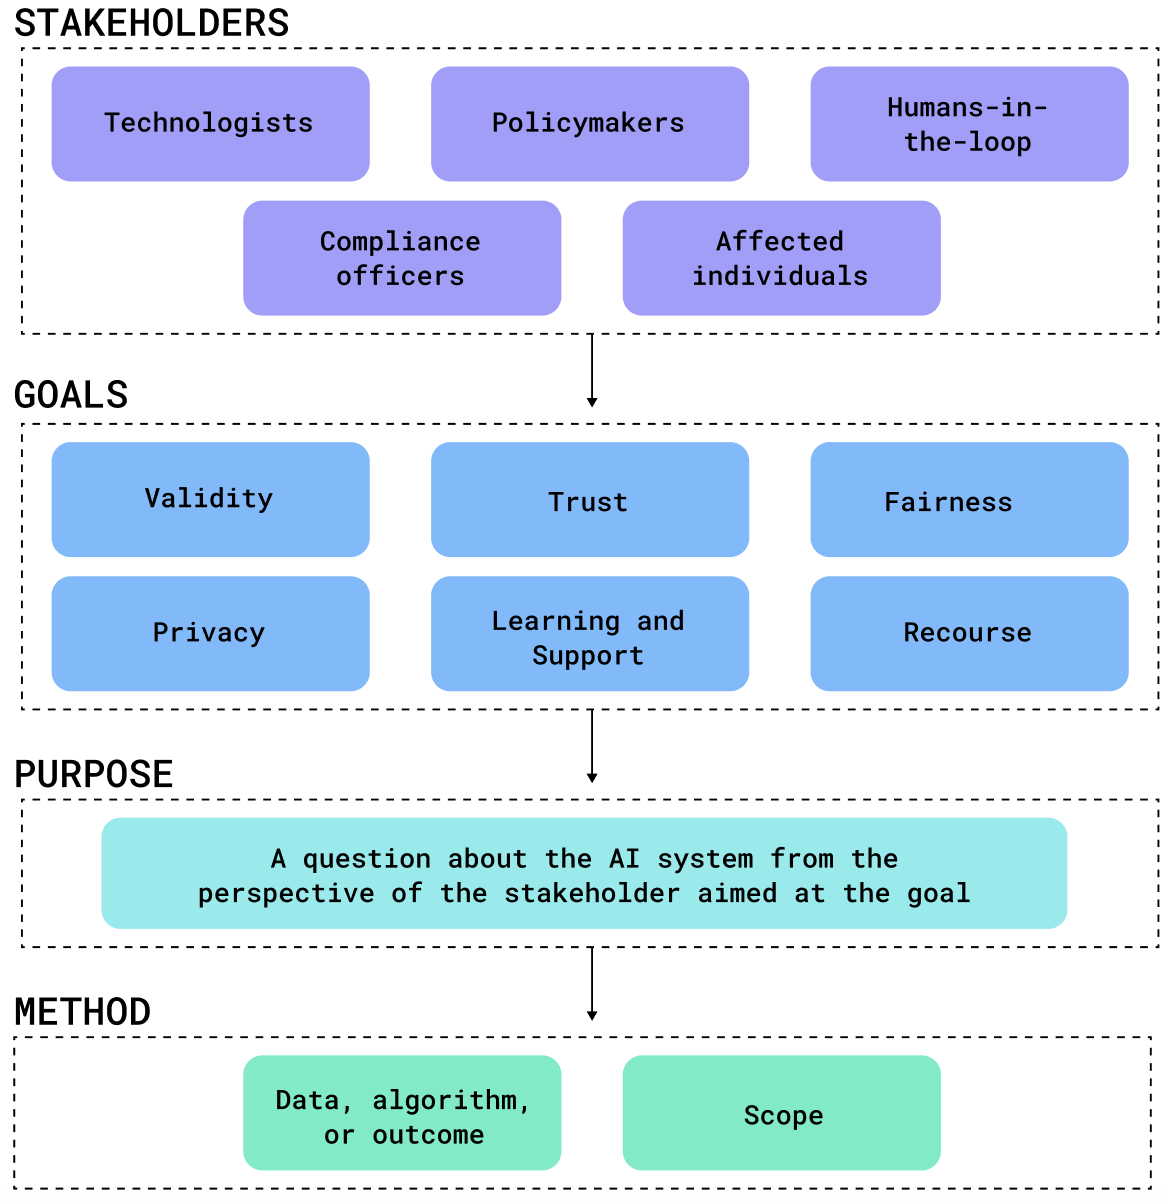
\includegraphics[width=1.0\linewidth]{figs/figure1.png}
    \end{center}
    \caption{A stakeholder-first approach for creating transparent ADS. The framework is made up of four components: stakeholders, goals, purpose, and methods. We recommend that transparency be thought of first by stakeholders, second by goals, before thirdly defining the purpose, and lastly choosing an appropriate method to serve said purpose. Using the framework is simple: starting at the top, one should consider each bubble in a component before moving onto the next component.}
    \label{fig:taxonomy}
\end{figure}

\begin{table*}[t]
\centering 
\begin{tabular}{p{0.12\textwidth}p{0.39\textwidth}p{0.39\textwidth}}
\toprule
\bf{Goal} & \bf{Definition} & \bf{Example} \\ \midrule
Validity & Making sure that an ADS is constructed correctly and is reasonable;  encompasses ideas like making sure the ADS is reliable and robust ~\cite{doshi2017towards} & An practitioner may use a transparency method to debug an ADS; An auditor may gain intuition about how an ADS is making decisions through transparency \\
Trust & Knowing ``how often an ADS is right'' and ``for which examples it is right'' ~\cite{lipton2018mythos}; influences the adoption of an ADS ~\cite{rodolfa2020machine} & A policymaker may use transparency to gain trust in the ADS; an affected individual may find through transparency that they \emph{do not} trust a particular ADS~\cite{schmidt2020transparency} \\
Fairness & Ensuring that an ADS is fair & An auditor may use an explanation about an ADS to make sure it is fair to all groups of individuals; a practitioner may use transparency tools to find bias in their modeling pipeline \\
Privacy & Ensuring that an ADS respects the data privacy of an individual & An auditor individual may use an explanation of the data used in an ADS to evaluate privacy concerns \\ 
Learning and Support &  To satisfy human curiosity, or increase understanding about how an ADS is supporting a real-world recommendation~\cite{rodolfa2020machine, molnar2019} & A doctor may use an explanation to understand an ADS recommendation of a certain treatment \\
Recourse & Allowing a stakeholder to take some action against the outcome of an ADS ~\cite{bhatt2020explainable, rodolfa2020machine} & An individual may use an explanation to appeal a loan rejection; An individual may request to see an explanation of an ADS output to understand why it was made \\
\bottomrule
\end{tabular}
\caption{Definitions and examples of stakeholder goals for the 6 categories of ADS transparency goals.}
\label{tab:goals}
\end{table*}
%\end{tabularx}

\subsubsection{Stakeholders} Much of ADS transparency research is focused on creating novel and innovative transparency methods for algorithms, and then later trying to understand how these methods can be used to meet stakeholders needs~\cite{bhatt2020explainable, preece2018stakeholders}. Counter to this rationale, we propose a starting point that focuses on ADS stakeholders: assuming algorithmic transparency is intended to improve the understanding of a human stakeholder, technologists designing transparent ADS must first consider the stakeholders of the system, before thinking about the system's goals or the technical methods for creating transparency.

The existing literature and taxonomies on ADS transparency have identified a number of important stakeholders, which include technologists, policymakers, auditors, regulators, humans-in-the-loop, and those individuals affected by the output of the ADS~\cite{DBLP:journals/corr/abs-2010-14374, meske, meyers2007street}.  While there is some overlap in how these stakeholders may think about transparency, in general, there is no single approach to designing transparent systems for these disparate stakeholder groups, and each of them has their own goals and purposes for wanting to understand an ADS~\cite{DBLP:journals/corr/abs-2001-09734}.  In fact, even within a stakeholder group there may be variations on how they define meaningful transparency~\cite{DBLP:conf/chi/HohmanHCDD19}. Designers of ADS may also want to weight the needs of separate stakeholders differently. For example, it may be more meaningful to meet the transparency needs of affected individuals over AI managers or auditors.

Importantly, by staking transparency on the needs of stakeholders, technologists will be compliant with citizen-aware regulations like the Right to Explanation, and those that require audits of ADS.

\emph{Running example.} In the ADS used by IEFP in Portugal, there are four main stakeholders: the technologists who developed the ADS, the policymakers who reviewed the ADS and passed laws for its implementation, the job counselors who use the system, and the affected individuals who are assessed for long-term unemployment.  In the development of the AI, explanations were created to meet the varying goals of many of these stakeholders including practitioners, policymakers, and the job counselors.  Unfortunately, and significantly, affected individuals were not considered.  Had the practitioners adopted a robust stakeholder-first approach to designing transparent systems they could have better considered how to meet the goals of this key stakeholder group. For example, a person may want to appeal being predicted low risk because they feel they are high risk for long-term unemployment and need access to better interventions.

%The variation in use-cases and goals of explanations by each stakeholder are captured in the next component of our approach, goals.

\subsubsection{Goals.} There has been little consensus in the literature on how ADS goals should be classified. Some researchers have focused broadly, classifying the goals of ADS as evaluating, justifying, managing, improving, or learning about the outcome of an ADS ~\cite{meske}.  Others have defined goals more closely to what can be accomplished by known transparency methods, including building trust, establishing causality, and achieving reliability, fairness, and privacy ~\cite{DBLP:journals/corr/abs-2012-01805}.  Amarasinghe et al. identified five main goals (designated as use-cases) of transparency specifically in a policy setting:  model-debugging, trust and adoption, whether or not to intervene, improving intervention assignments, and for recourse. In this context, the term intervention refers to a policy action associated with the outcome of an ADS.

Notably, the goals of transparency are distinct from the purpose. The purpose addresses a context-specific aim of the ADS. For example, if an explanation is created for an ADS with the purpose of explaining to an individual why their loan was rejected, the goal may be to offer individual recourse against the rejection. This distinction is made clear in~\ref{purpose}.

For our stakeholder-first approach we make two changes to the existing body of research work. First, we require that the goal of transparent design must start with a stakeholder. Since all transparency elements of an ADS are intended for a human audience, defining a stakeholder is implicit in defining goals. Second, we have established 6 goal categories, which encompass those found in literature.  These categories are validity, trust, learning and support, recourse, fairness and privacy, and are defined in Table~\ref{tab:goals} alongside concrete examples of how these goals may be implemented.

\begin{comment}
\begin{itemize}
    \item \textbf{Validity}.  Validity refers to making sure that an AI is constructed correctly and is reasonable.  It encompasses ideas like making sure the AI is reliable and robust ~\cite{doshi2017towards}.  %Validity may be achieved through model debugging. ~\cite{rodolfa2020machine}.
    \item \textbf{Trust}. In the context of an AI, trust refers knowing ``how often a model is right'' and ``for which examples it is right'' ~\cite{lipton2018mythos}.  Importantly, trust is related to the adoption of an ADS ~\cite{rodolfa2020machine}.
    \item \textbf{Learning and Support}.  Learning and support refers to when the goal of transparency in an ADS is to satisfy human curiosity, or increase understanding about how an AI is supporting a real-world recommendation~\cite{rodolfa2020machine, molnar2019}.
    \item \textbf{Recourse}.  Recourse refers to allowing a stakeholder to take some action against the outcome of an AI ~\cite{rodolfa2020machine}.
    \item \textbf{Fairness}.  Fairness refers to making sure that an AI is fair based on some metric, and transparency can be used to find bias within a model.
    \item \textbf{Privacy}.  Privacy refers to making sure that an AI respects the data privacy of an individual.  Transparency may be used to understand if privacy is being respected in an AI.
\end{itemize}
\end{comment}

An important discussion surrounding goals are the justifications for pursuing them.  For example, fairness and privacy goals may be justified for humanitarian reasons (they are perceived by the stakeholders as the ``right thing to do'').  Other justifications may be to prevent harm, like offering recourse to stakeholders against an outcome of an ADS, or for a reward, like an explanation that supports a doctor's correct diagnosis.  For reasons of scope we will not delve into the issue of goal justification in this paper.

\emph{Running example.} In our case study, transparency is built into the ADS with the goal of offering learning and support to job counselors. The ADS generates explanations about what factors contribute to an individual being classified as low, medium, or high risk for long-term unemployment, which job counselors use to help make better treatment decision.  Furthermore, the job counselor may also use the explanation to offer recommendations for recourse against a high risk score.

%Based on the SHAP factors displayed, the job counselor may choose to agree (or disagree) with the output of the AI, and assign (or not assign) the affected individual to the correct employment interventions.

\subsubsection{Purpose} \label{purpose}  Miller proposed that the purpose of transparency is to answer a ``why'' question ~\cite{DBLP:journals/corr/Miller17a}, and gives the following example: In the context where a system is predicting if a credit loan is accepted or rejected, one may ask, ``why was a particular loan rejected?'' Liao et al. expanded on this significantly by creating a ``question bank'' which is a mapping from a taxonomy of technical transparency methodology to different types of user questions.  Instead of just answering why questions, the works shows that transparency can be used to answer 10 categories of questions:  questions about the input, output, and performance of the system, how, why, why not, what if, how to be that, how to still be this, and others ~\cite{DBLP:conf/chi/LiaoGM20}. These questions have two important characteristics. First, they are context-specific and should address a direct transparency goal of the stakeholder. Second, and importantly for technologists, these questions can be mapped onto known methods for creating explanations, meaning that a well-defined purpose for transparency acts a bridge between the goals and methods.

Thoughtfully defining the goals and purpose of transparency in ADS is critical for technologists to be compliant with regulators. It is not sufficient to try and apply general, one-size-fits-all design like simply showing the features that were used by an ADS. For instance, both the proposed Algorithmic Accountability Act in the United States and the Artificial Intelligence Act in the European Union specifically mention that ADS should have transparency mechanisms that allow individuals to have recourse against a system outcome. Researchers have noted that feature-highlighting transparency lacks utility when there is a disconnect between the explanation and real-world actions~\cite{barocas2020hidden}. For instance, if someone is rejected for a loan and the reason for that decision is the person's age, there is no action that they can effectively take for recourse against that decision.

\emph{Running example.} In the long-term unemployment use case, there were two main purposes of transparency: to understand \emph{why} an individual was assigned to a particular risk category, and to understand \emph{what} could be done to help high risk individuals lower their chances of remaining long-term unemployed.

\subsubsection{Methods.}  Once the stakeholders, goals, and purposes for algorithmic transparency have been established, it is time for the technologist to pick the appropriate transparency method (somtimes called explainablity method). Over the past decade there has been significant work in transparent ADS research (sometimes called ``explainable AI'' research or XAI) on developing new methods for understanding opaque ADS.  There are several existing taxonomies of these methods, which show that explanations can be classified on a number of attributes like the scope (local or global), intrinsic or post-hoc, data or model, model-agnostic or model-specific, surrogate or model behavior, and static or interactive ~\cite{DBLP:journals/jmlr/AryaBCDHHHLLMMP20, molnar2019, DBLP:journals/corr/abs-2012-01805}. Furthermore, researchers have created a number of different tools to accomplish transparency in ADS~\cite{DBLP:conf/nips/LundbergL17, ribeiro2016should, datta2016algorithmic, DBLP:journals/corr/abs-2004-00668, DBLP:journals/corr/abs-2004-00668}.

In contrast to the complex classification of transparency methods by technologists, regulations have focused on two elements of ADS: (1) what aspect of the ADS pipeline is being explained (the data, algorithm, or outcome)?, and (2) what is the scope of the explanation (for one individual or the entire system)? Table \ref{tab:laws} shows how different regulations speak to different combinations of pipeline and scope. In our stakeholder first-approach to transparency, we focus on these two main attributes. We will not discuss specific methods in detail, but for the convenience of technologists we have underlined them throughout this discussion.

\begin{table*}[]
\centering
\begin{tabular}{m{0.07\textwidth}m{0.24\textwidth}m{0.24\textwidth}m{0.24\textwidth}}
\toprule
 & \bf{Data} & \bf{Algorithm} & \bf{Outcome} \\
\midrule
\multicolumn{1}{l}{\bf{Local}}  & GDPR (EU) gives individuals the right to request a copy of any of their personal data & Right to Explanation gives individuals the right to know how an algorithm made a decision about them  & Both the proposed Algorithmic Accountability Act (US) and Artificial Intelligence Act (AI) give individuals the right to recourse \\
\multicolumn{1}{l}{\bf{Global}} & OPEN Government Data Act (US) mandates the government publishes public data & EU Regulation 2019/115 requires that online stores and search engines to disclose the algorithmic parameters used to rank goods and services on their site & NYC Int 1894-2020 requires hiring algorithms be audited for biased outcomes \\
\bottomrule
\end{tabular}
\caption{How different laws regulate the aspects the ADS pipeline (the data, algorithm or outcome), and within what scope (local or global).}
\label{tab:laws}
\end{table*}

\textbf{Data, algorithm, or outcome.} Transparency methods have focused on generating explanations for three different ``points in time'' in an ADS pipeline:  the data (pre-processing), the model/algorithm (in-processing, intrinsic), or the outcome (post-processing, post-hoc) ~\cite{DBLP:journals/jmlr/AryaBCDHHHLLMMP20, ventocilla2018towards}.  Importantly, transparency is relevant for each part of the machine learning pipeline because issues likes bias can arise within each component ~\cite{yang2020fairness}.

Transparency techniques that focus on the pre-processing component of the pipeline, that is, on the data used to create an ADS, typically include descriptive statistics or data visualizations.\\  
\underline{Data visualizations} have proved useful for informing users and making complex information more accessible and digestible, and have even been found to have a powerful persuasive effect ~\cite{DBLP:journals/tvcg/PandeyMNSB14, tal2016blinded}. Therefore, it is advisable to use data visualization if it can easily  address the purpose of an explanation. However, visualizations should be deployed thoughtfully, as they have the ability to be abused and can successfully misrepresent a message through techniques like exaggeration or understatement ~\cite{pandey2015deceptive}.

Techniques for creating in-processing or post-processing explanations call into question the important consideration of using explainable versus black-box algorithms when designing AI. The machine learning community accepts two classifications of models:  those that are intrinsically transparent by their nature (sometimes called directly interpretable or white-box models), and those that are not (called black box models) ~\cite{DBLP:journals/corr/abs-2012-01805}. Interpretable models, like linear regression, decision trees, or rules-based models, have \underline{intrinsic transparency mechanisms} that offer algorithmic transparency, like the linear formula, the tree diagram, and the set of rules, respectively. There are also methods like \underline{\emph{select-regress-round}} that simplify black-box models into interpretable models that use a similar set of features~\cite{jung2017simple}.

%It’s worth noting that there is no rigorous distinction between these two groups of models; instead, a set of models have been accepted as explainable and data scientists seem to ``know them when they see them.''

As an important design consideration for technologists, researchers have studied the effect of the complexity of a model and how it impacts its ability to be understood by a stakeholder. A user study found that the understanding of a machine learning model is negatively correlated with it's complexity, and found decision trees to be among the model types most understood by users ~\cite{DBLP:conf/scai/AllahyariL11}. An additional, lower-level design consideration is that model complexity is not fixed to a particular model type, but rather to the way that the model is constructed. For example, a decision tree with 1,000 nodes will be understood far less well than a tree with only 3 or 5 nodes.

In contrast to in-process transparency, which is intrinsically built into a model or algorithm, post-hoc transparency aims to answer questions about a model or algorithm after is has already been created.  Some of the most popular post-hoc methods are \underline{LIME, SHAP, SAGE, and QII}~\cite{DBLP:conf/nips/LundbergL17, ribeiro2016should, datta2016algorithmic, DBLP:journals/corr/abs-2004-00668}. These methods are considered \emph{model-agnostic} because they can be used to create explanations for any model, from linear models to random forests to neural networks. Some methods create a transparent \emph{surrogate model} that mimics the behavior of a black-box model. For example, \underline{LIME} creates a linear regression to approximate an underlying black-box model~\cite{DBLP:conf/nips/LundbergL17}. More work needs to be done in this direction, but one promising study has shown that post-hoc explanations can actually improve the perceived trust in the outcome of an algorithm ~\cite{DBLP:conf/softcomp/BekriKH19}.

%Arguably, adding layers onto black box models can compound their complexity, rather than reduce it.
However, post-hoc transparency methods have been shown to have two weaknesses that technologists should be aware of: (1) in many cases, these methods are at-best \emph{approximations} of the black-box they are trying to explain ~\cite{zhang2019should}, and (2) these methods may be vulnerable to adversarial attacks and exploitation ~\cite{DBLP:conf/aies/SlackHJSL20}.  Some researchers have also called into question the utility of black-box models and post-hoc explanation methods altogether, and have cautioned against their use in real-world contexts like clinical settings ~\cite{rudin2019stop}.  %However, a notable shortcoming in this study is that it focuses on precieved trust of a stakeholder, and not their understanding or how it could effect their goals in using the explanation.

\textbf{Scope}\label{subsec:scope}. There are two levels at which a transparent explanation about an ADS can operate:  it either explains its underlying algorithm fully, called a ``global'' explanation; or it explains how the algorithm operates on one specific instance, called a ``local'' explanation. Molnar further subdivides each of these levels into two sub-levels: global explanations can either be holistic (applying to an entire algorithm, which includes all of its features, and in the case of an ensemble algorithm, all of the component algorithms) or modular, meaning they explain on part of the holistic explanation and local explanations can either be applied to a single individual, or aggregated to provide local explanations for an entire group ~\cite{molnar2019}.

The scope of an explanation is highly relevant to the stakeholder and goals of an explanation, and is related to whether the stakeholder operates at a system or individual level. Researchers found that the scope of explanation can influence whether or not an individual thinks a model is fair~\cite{DBLP:journals/corr/abs-2101-09429,DBLP:conf/chi/LiaoGM20}. Policymakers and ADS compliance officers are more apt to be concerned with system level goals, like ensuring that the ADS is fair, respects privacy, and is valid overall, while humans-in-the-loop and those individuals affected by the outcome of an ADS are likely more interested in seeing local explanations to pertain to their specific cases. Technologists should consider both.

Naturally, there is considerable overlap between stakeholders' scope needs (for example, an auditor may want to inspect a model globally and look at local cases), but generally, \textit{it is important} which scope an explanation has.  Therefore designers of ADS explanations should be thoughtful of how they select the scope of an explanation based on a stakeholder and their goals.

\emph{Running-example.} In the IEFP use case, SHAP factors were given to job counselors to show the top factors influencing the score of a candidate both positively and negatively~\cite{zejnilovic2020algorithmic}. The transparency provided by SHAP provided a local explanation about the outcome of the model. A bias audit was also conducted on the entire algorithm, and presented to policy officials within IEFP.

Overall, researchers found that the explanations improved the confidence of the decisions, but counter-intuitively, had a somewhat negative effect on the quality of those decisions~\cite{zejnilovic2020algorithmic}.

\subsection{Putting the Approach into Practice}
The stakeholder-first approach describe in Section~\ref{sec:approach} is meant to act as a guide for technologists creating regulatory-compliant ADS. Putting this approach into practice is simple: starting at the first component in Figure~\ref{fig:taxonomy} (\emph{stakeholders}), one should consider each bubble, before moving onto the next component and again considering each bubble. By the time one has finished worked their way through the figure, they should have considered all the possible \emph{stakeholders}, \emph{goals}, \emph{purposes}, and \emph{methods} of an ADS. An instantiation of the approach can be found throughout Section~\ref{sec:approach} in the running example of building an ADS that predicts the risk of long-term unemployment in Portugal.

It's important to note that our proposed stakeholder-first approach is only a high-level tool for thinking about ADS transparency through the perspective of stakeholders and their needs. Beyond this approach, there are meaningful low-level steps that can be taken by technologists when it comes to actually implement transparency into ADS. One such step is the use of \emph{participatory design}, where stakeholders are included directly in design conversations~\cite{eiband2018bringing, cech2021tackling, aizenberg2020designing, gupta2020participatory}. In one promising study researchers used participatory design to successfully create better algorithmic explanations for users in the field of communal energy accounting~\cite{cech2021tackling}.

%\subsubsection{Design Considerations}

%When implementing
%It has also been shown that, counterintuitively, giving more information for an explanation of a ML model can actually decrease the perceived understanding of a stakeholder – the stakeholder may become confused or less satisfied due to an overload of information ~\cite{DBLP:conf/chi/LiaoGM20, narayanan2018humans}.  Below we discuss several attributes of methods for explaining AI and how they map onto stakeholder needs.



